\documentclass[../../../main.tex]{subfiles}
\begin{document}

%%%%%%%%%%%%%%%%%%%%%%%%%%%%%%%%%%%%%%%%%
%%%%%%%%%%%%%%%%%%%%%%%%%%%%%%%%%%%%%%%%%
%%%%%%%%%%%%%%%%%%%%%%%%%%%%%%%%%%%%%%%%%
\chapter{Hypothesis testing introduction}

Suppose a very large franchised brand called McCallister Logistics releases a statement which claims that all female McCallister employees are paid on average a salary of \$55K or more per yer. We would like to determine if this is correct. 

Of course, we do not know the actual population mean (the actual average salary of female employees). But suppose also that the McCallister parent company doesn't know it either (the brand is so large that it is impossible to get a completely accurate picture of all franchisee operations).

Fortunately, we can test McCallister's claim by taking a sample of female employees, and we can check to see if the mean of our sample lines up with McCallister's claim. Being good statisticians, we will follow a certain procedure to do this.


%%%%%%%%%%%%%%%%%%%%%%%%%%%%%%%%%%%%%%%%%
%%%%%%%%%%%%%%%%%%%%%%%%%%%%%%%%%%%%%%%%%
\section{The null hypothesis}

As good statisticians, we will take the ``innocent until proven guilty'' approach. Let us treat McCallister's claim as the current best working hypothesis. That is to say, let us assume it to be correct, unless we find very strong evidence to overturn it. 

In statistics, we call McCallister's claim the \vocab{null hypothesis}. We also call it the \vocab{status quo}. Both of these names are meant to convey the idea that this is the hypothesis that we consider to be given, which we assume to be correct, unless we find strong evidence to overturn it.

We use a special symbol to refer to the null hypothesis. We write it like this:

\begin{equation*}
  \NullHyp/
\end{equation*}

\noindent
So, the hypothesis that we start with here (our null hypothesis) is McCallister's claim that all female employees earn on average \$55K or more per year. Let us extract what we can say about this claim, in statistical terms:

\begin{itemize}
  \item The population we are interested in is all female employees who work under the McCallister brand.
  \item The random variable $\RandVar/$ we are interested in is the salary of a female employee.
  \item The values that $\RandVar/$ can take on are monetary values, i.e., \$55K, or \$56,750, or \$63,786.23, and so on.
  \item The population parameter we are interested in is the mean salary of the population, i.e., $\populationmean$ of $\RandVar/$.
  \item The claim that McCallister is making is that the population mean $\populationmean$ is equal to or greater than \$55K, i.e., $\populationmean \geq 55,000$.
\end{itemize}

\noindent
Remember that McCallister does not know the actual mean of the population. So in effect, by making this claim, they are \emph{proposing} a mean. They are \emph{hypothesizing} what they think it is. Let us use a special symbol to stand for this hypothesized mean:

\begin{equation*}
  \HypPopMean/
\end{equation*}

\noindent
We put a subscripted zero on it to indicate that this is the \emph{hypothesized} mean. It is the mean that is coming along with the null hypothesis $\NullHyp/$, which also has a subscripted zero. The subscripted zero is important, because it distinguishes the hypothesized mean from the actual mean. And remember that we symbolize the actual population mean without a subscripted zero. Like this:

\begin{equation*}
  \populationmean
\end{equation*}

\noindent
With these symbols at hand, we can state the null hypothesis exactly:

\begin{equation*}
  \NullHyp/: \populationmean \geq \HypPopMean/
\end{equation*}

\noindent
Read this as follows: ``The null hypothesis $\NullHyp/$ claims that the true population mean $\populationmean$ is greater than or equal to the hypothesized population mean $\HypPopMean/$,'' where the hypothesized population mean $\HypPopMean/$ is 55,000.


%%%%%%%%%%%%%%%%%%%%%%%%%%%%%%%%%%%%%%%%%
%%%%%%%%%%%%%%%%%%%%%%%%%%%%%%%%%%%%%%%%%
\section{The alternative hypothesis}

For every null hypothesis, here is a corresponding \vocab{alternative hypothesis}, which is the contradictory opposite of the null hypothesis. We use a special symbol to stand for the alternative hypothesis:

\begin{equation*}
  \AltHyp/
\end{equation*}

\noindent
What's the contradictory opposite? Well, the null hypothesis is this:

\begin{equation*}
  \NullHyp/: \populationmean \geq \HypPopMean/
\end{equation*}

\noindent
And since this claims that the true population mean is \emph{greater than or equal to} the hypothesized population mean, then the opposite claim must be that the true population mean is \emph{less than} the hypothesized mean. That is:

\begin{equation*}
  \AltHyp/: \populationmean < \HypPopMean/
\end{equation*}

\noindent
These two hypothesis --- $\NullHyp/$ and $\AltHyp/$ --- are opposites, and they encompass all possibilities. Either the true population mean is 55K or greater (in which case $\NullHyp/$ is correct), or the true population mean is less than that (in which case $\AltHyp/$ is correct).


%%%%%%%%%%%%%%%%%%%%%%%%%%%%%%%%%%%%%%%%%
%%%%%%%%%%%%%%%%%%%%%%%%%%%%%%%%%%%%%%%%%
\section{Confirming with a sample}

As noted earlier, we will take the ``innocent until proven guilty'' approach, and assume that the null hypothesis is true. To test the null hypothesis, we will take a sample, and we will calculate the mean $\samplemean{x}$ of that sample, and then we will check to see if that sample mean $\samplemean{x}$ confirms or refutes the null hypothesis. 

What would we expect to see, to confirm that the null hypothesis is correct? Let us consider some examples, and visualize them. First, let us mark the hypothesized population mean on a plot (numbers are in thousands, so that 55 really means 55,000):

\begin{center}
  \begin{tikzpicture}
    \begin{axis}[
      axis lines*=left,
      ytick=\empty,
      height=5cm,
      width=12cm,
      enlarge y limits={value=0.2,upper},
      ]
      \addplot[smooth, fill=none, domain=40:70] 
        coordinates{((55, 0) (55, 10)}
        \closedcycle;

      % \draw (55, 0) -- (55, 10);
      \node at (55, 6.5) [label=right:{$\HypPopMean/ = 55$}] {};

    \end{axis}
  \end{tikzpicture}
\end{center}

\noindent
Now suppose that we take a sample. We select 30 female employees under the McCallister brand, and we take the average (the mean $\samplemean{x}$) of their salaries. Suppose it turns out to be 66K. Let's mark that:

\begin{center}
  \begin{tikzpicture}
    \begin{axis}[
      axis lines*=left,
      ytick=\empty,
      height=5cm,
      width=12cm,
      enlarge y limits={value=0.2,upper},
      ]
     \addplot[smooth, fill=lightgray, domain=40:85] 
        coordinates{
          (55, 0) (55, 10)}
        \closedcycle;

      \draw (55, 0) -- (55, 10);
      \node at (55, 6.5) [label=right:{$\HypPopMean/ = 55$}] {};

     \addplot[smooth, color=red, domain=40:85] 
        coordinates{
          (66, 0) (66, 10)}
        \closedcycle;

      \draw[color=red] (66, 0) -- (66, 10);
      \node at (66, 6.5) [label=left:{$\samplemean{x} = 66$}] {};

    \end{axis}
  \end{tikzpicture}
\end{center}

\noindent
Does this confirm, or refute the null hypothesis? It confirms it. We know from the \CLT/ that sample means cluster around the true population mean in a normal shape. This particular sample mean of 66 must come from the true population's sample distribution, because we sampled it from the real population! So we know that the true population mean must be somewhere around 66, because 66 must be part of the true population's sampling distribution. 

For example, the true population mean could be a little to the right of our sample mean 66. It could be at (say) 68:

\begin{center}
  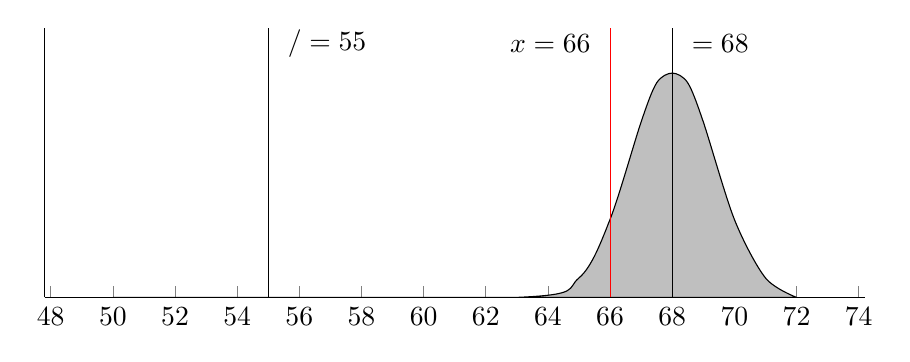
\begin{tikzpicture}
    \begin{axis}[
      axis lines*=left,
      ytick=\empty,
      height=5cm,
      width=12cm,
      enlarge y limits={value=0.2,upper},
      ]

      \draw (55, 0) -- (55, 10);
      \node at (55, 6.5) [label=right:{$\HypPopMean/ = 55$}] {};

     \addplot[smooth, fill=lightgray, domain=40:85] 
        coordinates{
          (50, 0)
          (63, 0) (65, 0.5) (66, 2) (67, 4.5) (67.5, 5.5)
          (68, 5.75)
          (68.5, 5.5) (69, 4.5) (70, 2) (71, 0.5) (72, 0)}
        \closedcycle;

      \draw (68, 0) -- (68, 10);
      \node at (68, 6.5) [label=right:{$\populationmean = 68$}] {};

      \draw[color=red] (66, 0) -- (66, 10);
      \node at (66, 6.5) [label=left:{$\samplemean{x} = 66$}] {};

    \end{axis}
  \end{tikzpicture}
\end{center}

\noindent
Alternatively, the true population mean could be to the left of 66. Perhaps the sample we took just happens to be a sample of all the highest salaried females under the McCallister brand. Then the sample that we just happened to get (entirely by chance) is in the very right tail of the true population's sampling distribution:

\begin{center}
  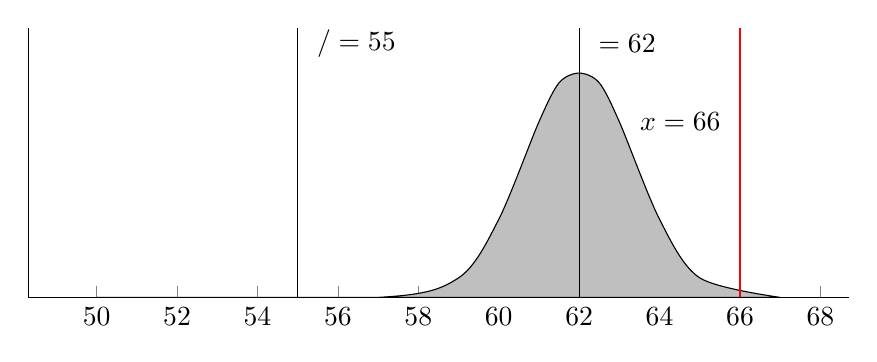
\begin{tikzpicture}
    \begin{axis}[
      axis lines*=left,
      ytick=\empty,
      height=5cm,
      width=12cm,
      enlarge y limits={value=0.2,upper},
      ]

      \draw (55, 0) -- (55, 10);
      \node at (55, 6.5) [label=right:{$\HypPopMean/ = 55$}] {};

     \addplot[smooth, fill=lightgray, domain=40:85] 
        coordinates{
          (50, 0)
          (57, 0) (59, 0.5) (60, 2) (61, 4.5) (61.5, 5.5)
          (62, 5.75)
          (62.5, 5.5) (63, 4.5) (64, 2) (65, 0.5) (67, 0)}
        \closedcycle;

      \draw (62, 0) -- (62, 10);
      \node at (62, 6.5) [label=right:{$\populationmean = 62$}] {};

      \draw[color=red] (66, 0) -- (66, 10);
      \node at (66, 4.5) [label=left:{$\samplemean{x} = 66$}] {};

    \end{axis}
  \end{tikzpicture}
\end{center}

\noindent
This would still confirm the null hypothesis. We can see that even if our sample is in the far right tail of the true population's sampling distribution, the true population's sampling distribution is still very far to the right of the hypothesized mean of 55K. 

Again, we don't know where the true population mean is. All we know is the mean of the sample we took. But we know from the \CLT/ that all possible samples cluster around the true population mean in a normal shape. And we know that the sample we took must come from the true population's sampling distribution, because we sampled it from the real population! 

So we know that our sample mean of 66 \emph{must} be included in the true population mean, and we can see that no matter where the true population mean is, it is still going to be to the right of the hypothesized mean of 55. Hence, this sample confirms the null hypothesis, which claims that the true population mean is going to be greater than or equal to 55K.


%%%%%%%%%%%%%%%%%%%%%%%%%%%%%%%%%%%%%%%%%
%%%%%%%%%%%%%%%%%%%%%%%%%%%%%%%%%%%%%%%%%
\section{Refuting with a sample}

Let's consider a case now where we get a sample that definitively refutes the null hypothesis. Again, here is the proposed population mean, at 55K:

\begin{center}
  \begin{tikzpicture}
    \begin{axis}[
      axis lines*=left,
      ytick=\empty,
      height=5cm,
      width=12cm,
      enlarge y limits={value=0.2,upper},
      ]
      \addplot[smooth, fill=none, domain=40:70] 
        coordinates{((55, 0) (55, 10)}
        \closedcycle;

      % \draw (55, 0) -- (55, 10);
      \node at (55, 6.5) [label=left:{$\HypPopMean/ = 55$}] {};

    \end{axis}
  \end{tikzpicture}
\end{center}

\noindent
Suppose now that we take a sample of 30 female employees under the McCallister brand, and we average their salaries, and we find that their average salary is 44K. Let's mark it:

\begin{center}
  \begin{tikzpicture}
    \begin{axis}[
      axis lines*=left,
      ytick=\empty,
      height=5cm,
      width=12cm,
      enlarge y limits={value=0.2,upper},
      ]
     \addplot[smooth, fill=lightgray, domain=40:85] 
        coordinates{
          (55, 0) (55, 10)}
        \closedcycle;

      \draw (55, 0) -- (55, 10);
      \node at (55, 6.5) [label=right:{$\HypPopMean/ = 55$}] {};

     \addplot[smooth, color=red, domain=40:85] 
        coordinates{
          (44, 0) (44, 10)}
        \closedcycle;

      \draw[color=red] (44, 0) -- (44, 10);
      \node at (44, 6.5) [label=left:{$\samplemean{x} = 44$}] {};

    \end{axis}
  \end{tikzpicture}
\end{center}

\noindent
Does this sample confirm or refute the null hypothesis? In this case, it definitively refutes it. As before, the sample mean must come from the real population sampling distribution (because we took our sample from the real population), and we know from the \CLT/ that all possible sample means will cluster around the true population mean in a normal shape.

So, the true population mean must be somewhere around 44, and 44 must be one of the possible values in the curve. For example, it could be that the true population mean is 46:

\begin{center}
  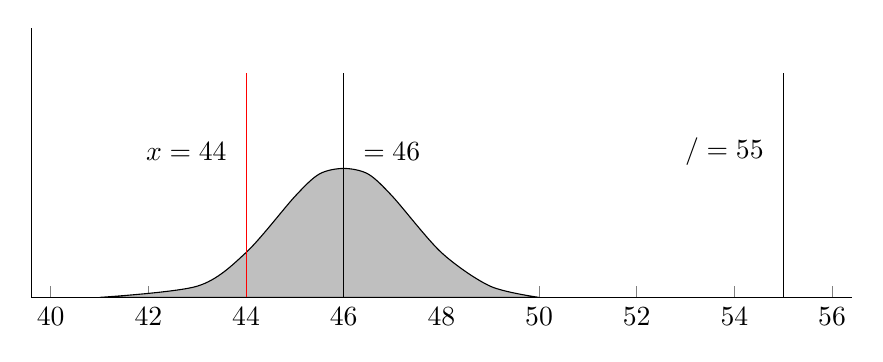
\begin{tikzpicture}
    \begin{axis}[
      axis lines*=left,
      ytick=\empty,
      height=5cm,
      width=12cm,
      enlarge y limits={value=0.2,upper},
      ]

      \draw (55, 0) -- (55, 10);
      \node at (55, 6.5) [label=left:{$\HypPopMean/ = 55$}] {};

     \addplot[smooth, fill=lightgray, domain=40:85] 
        coordinates{
          (41, 0) (43, 0.5) (44, 2) (45, 4.5) (45.5, 5.5)
          (46, 5.75)
          (46.5, 5.5) (47, 4.5) (48, 2) (49, 0.5) (50, 0)}
        \closedcycle;

     \addplot[smooth, color=black, domain=40:85] 
        coordinates{
          (55, 0) (55, 10)}
        \closedcycle;

      \draw (46, 0) -- (46, 10);
      \node at (46, 6.5) [label=right:{$\populationmean = 46$}] {};

      \draw[color=red] (44, 0) -- (44, 10);
      \node at (44, 6.5) [label=left:{$\samplemean{x} = 44$}] {};

    \end{axis}
  \end{tikzpicture}
\end{center}

\noindent
We can see from the picture that the true population mean is certainly going to be lower than the proposed mean of 55K. Even if, entirely by chance, we managed to select the 30 lowest paid female employees, so that our sample mean of 44 represents the lowest possible salary sample, we are still able to see in the picture that even then the true population mean would still be below 55:

\begin{center}
  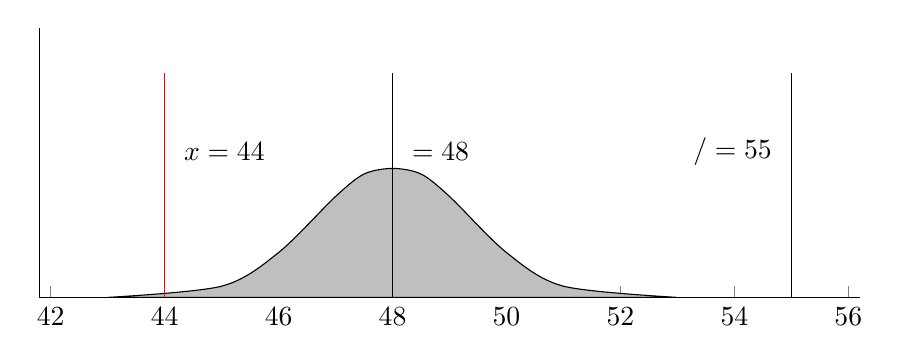
\begin{tikzpicture}
    \begin{axis}[
      axis lines*=left,
      ytick=\empty,
      height=5cm,
      width=12cm,
      enlarge y limits={value=0.2,upper},
      ]

      \draw (55, 0) -- (55, 10);
      \node at (55, 6.5) [label=left:{$\HypPopMean/ = 55$}] {};

     \addplot[smooth, fill=lightgray, domain=40:85] 
        coordinates{
          (43, 0) (45, 0.5) (46, 2) (47, 4.5) (47.5, 5.5)
          (48, 5.75)
          (48.5, 5.5) (49, 4.5) (50, 2) (51, 0.5) (53, 0)}
        \closedcycle;

     \addplot[smooth, color=black, domain=40:85] 
        coordinates{
          (55, 0) (55, 10)}
        \closedcycle;

      \draw (48, 0) -- (48, 10);
      \node at (48, 6.5) [label=right:{$\populationmean = 48$}] {};

      \draw[color=red] (44, 0) -- (44, 10);
      \node at (44, 6.5) [label=right:{$\samplemean{x} = 44$}] {};

    \end{axis}
  \end{tikzpicture}
\end{center}

\noindent
So a sample of 44 refutes the null hypothesis, because it shows that the true population must be below 55, which contradicts the null hypothesis's claim that the true population is 55K or greater.


%%%%%%%%%%%%%%%%%%%%%%%%%%%%%%%%%%%%%%%%%
%%%%%%%%%%%%%%%%%%%%%%%%%%%%%%%%%%%%%%%%%
\section{Ambiguous cases}

We visualized a case where a sample mean was so far to the right of the hypothesized mean $\HypPopMean/$ of 55 that it definitively confirmed the null hypothesis, and we visualized a case where the sample mean was so far to the left that it definitively refuted the null hypothesis. 

Things get trickier when the sample mean turns out to be much closer to the hypothesized mean. Suppose, for example, that we take a sample of 30 female salaries, and we get a sample mean of 52:

\begin{center}
  \begin{tikzpicture}
    \begin{axis}[
      axis lines*=left,
      ytick=\empty,
      height=5cm,
      width=12cm,
      enlarge y limits={value=0.2,upper},
      ]
     \addplot[smooth, fill=lightgray, domain=45:65] 
        coordinates{
          (55, 0) (55, 10)}
        \closedcycle;

      \draw (55, 0) -- (55, 10);
      \node at (55, 6.5) [label=right:{$\HypPopMean/ = 55$}] {};

      \draw[color=red] (52, 0) -- (52, 4.5);
      \node at (52, 4.5) [label=above:{$\samplemean{x} = 52$}] {};

    \end{axis}
  \end{tikzpicture}
\end{center}

\noindent
Now, the true population could be centered exactly at 55K, as McCallister claims, and 52 would be within the sampling distribution:

\begin{center}
  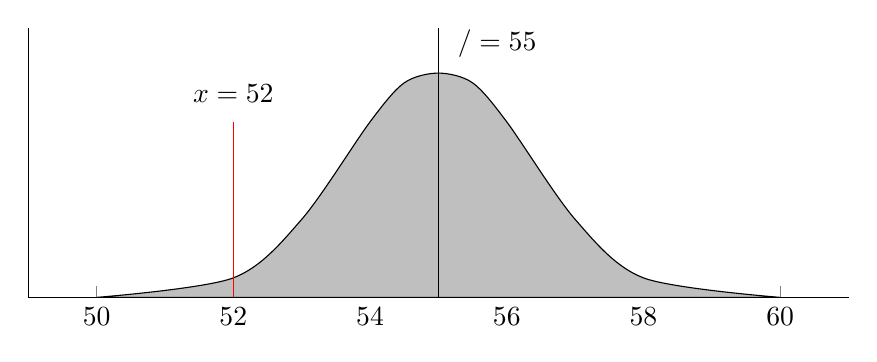
\begin{tikzpicture}
    \begin{axis}[
      axis lines*=left,
      ytick=\empty,
      height=5cm,
      width=12cm,
      enlarge y limits={value=0.2,upper},
      ]
      \addplot[smooth, fill=lightgray, domain=45:65] 
        coordinates{
          (50, 0) (52, 0.5) (53, 2) (54, 4.5) (54.5, 5.5)
          (55, 5.75)
          (55.5, 5.5) (56, 4.5) (57, 2) (58, 0.5) (60, 0)} 
        \closedcycle;

      \draw (55, 0) -- (55, 10);
      \node at (55, 6.5) [label=right:{$\HypPopMean/ = 55$}] {};

      \draw[color=red] (52, 0) -- (52, 4.5);
      \node at (52, 4.5) [label=above:{$\samplemean{x} = 52$}] {};

    \end{axis}
  \end{tikzpicture}
\end{center}

\noindent
But the population mean could be centered at, say 50. A sample mean of 52 is a perfectly reasonable sample to draw from that population:

\begin{center}
  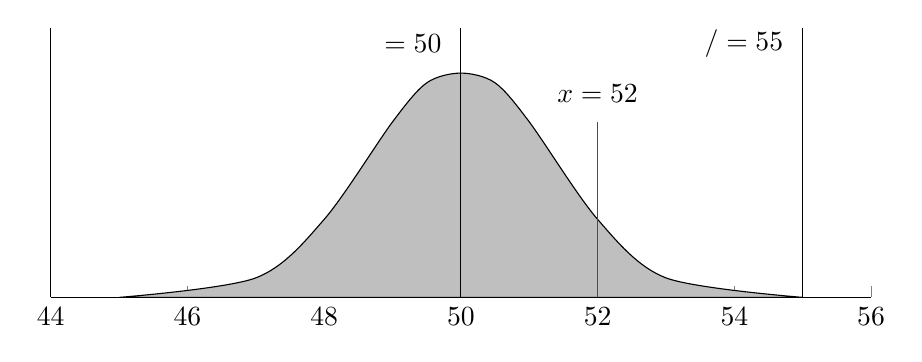
\begin{tikzpicture}
    \begin{axis}[
      axis lines*=left,
      ytick=\empty,
      height=5cm,
      width=12cm,
      enlarge y limits={value=0.2,upper},
      ]
      \addplot[smooth, fill=lightgray, domain=45:65] 
        coordinates{
          (45, 0) (47, 0.5) (48, 2) (49, 4.5) (49.5, 5.5)
          (50, 5.75)
          (50.5, 5.5) (51, 4.5) (52, 2) (53, 0.5) (55, 0)} 
        \closedcycle;

      \draw (50, 0) -- (50, 10);
      \node at (50, 6.5) [label=left:{$\populationmean = 50$}] {};

      \draw (55, 0) -- (55, 10);
      \node at (55, 6.5) [label=left:{$\HypPopMean/ = 55$}] {};

      \draw[color=red] (52, 0) -- (52, 4.5);
      \node at (52, 4.5) [label=above:{$\samplemean{x} = 52$}] {};

    \end{axis}
  \end{tikzpicture}
\end{center}

\noindent
So in this case, we have taken a sample that doesn't definitively confirm or refute the null hypothesis. What do we do then?


%%%%%%%%%%%%%%%%%%%%%%%%%%%%%%%%%%%%%%%%%
%%%%%%%%%%%%%%%%%%%%%%%%%%%%%%%%%%%%%%%%%
\section{Draw a line in the sand}

As good statisticians, we take the following stance. We take the ``innocent until proven guilty'' approach, and so we will assume that the null hypothesis will stand, unless we have sufficient evidence to overturn it. 

What counts as ``sufficient evidence'' to overturn the null hypothesis? Well, we have to draw a line on the plot, and say that this line is the threshold. We call this line the \vocab{critical point}, or the \vocab{level of significance}, or just \vocab{alpha} (for reasons that will become clear soon).

The critical point serves as a decision threshold. We use it like this: if we get a sample mean that is lower than the critical point, then that sample counts as sufficient evidence to overturn the null hypothesis. If we get a sample that is larger than the critical point, then we will say that the evidence is simply not strong enough to persuade us to overturn the status quo (the null hypothesis).

We call the area to the right of $\alpha$ the \vocab{non-rejection} region, because it is the area where, if we get a sample from there, we do not reject the null hypothesis. By contrast, the area to the left of $\alpha$ is called the \vocab{rejection} rejection.

For example, suppose we decide to put alpha right at 50 on the plot:

\begin{center}
  \begin{tikzpicture}
    \begin{axis}[
      axis lines*=left,
      ytick=\empty,
      height=5cm,
      width=12cm,
      enlarge y limits={value=0.2,upper},
      ]
     \addplot[smooth, fill=lightgray, domain=45:65] 
        coordinates{
          (55, 0) (55, 10)}
        \closedcycle;

      \draw (55, 0) -- (55, 10);
      \node at (55, 6.5) [label=right:{$\HypPopMean/ = 55$}] {};

      \draw[color=blue] (50, 0) -- (50, 10);
      \node at (50, 6.5) [label=left:{$\alpha = 50$}] {};

    \end{axis}
  \end{tikzpicture}
\end{center}

\noindent
Now we can say that any sample mean that is smaller than $\alpha$ counts as strong enough evidence to overturn the null hypothesis, but any sample mean that is bigger than $\alpha$ is not strong enough.

Let's look at some examples. Suppose that the true population mean is centered exactly at 55, just as the null hypothesis proposes:

\begin{center}
  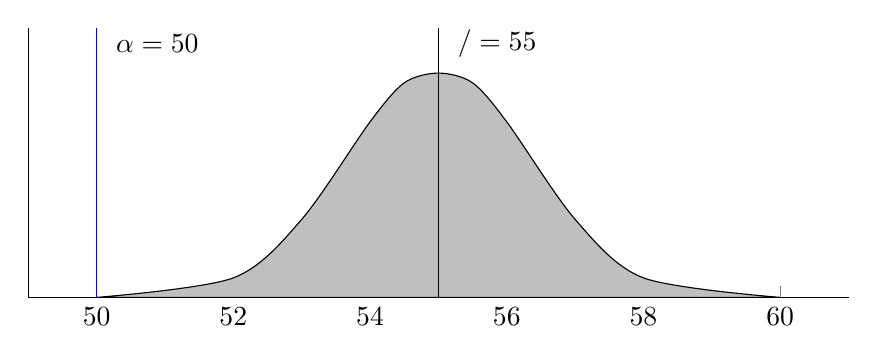
\begin{tikzpicture}
    \begin{axis}[
      axis lines*=left,
      ytick=\empty,
      height=5cm,
      width=12cm,
      enlarge y limits={value=0.2,upper},
      ]
      \addplot[smooth, fill=lightgray, domain=45:65] 
        coordinates{
          (50, 0) (52, 0.5) (53, 2) (54, 4.5) (54.5, 5.5)
          (55, 5.75)
          (55.5, 5.5) (56, 4.5) (57, 2) (58, 0.5) (60, 0)} 
        \closedcycle;

      \draw (55, 0) -- (55, 10);
      \node at (55, 6.5) [label=right:{$\HypPopMean/ = 55$}] {};

      \draw[color=blue] (50, 0) -- (50, 10);
      \node at (50, 6.5) [label=right:{$\alpha = 50$}] {};

    \end{axis}
  \end{tikzpicture}
\end{center}

\noindent
If the true population mean is really centered at 55, then we know from the \CLT/ that any sample we could possibly take will have a mean that falls in the grey area. And since any value inside the grey is greater than $\alpha$, we will conclude that such a sample does not give us enough evidence to overturn the null hypothesis. So, the null hypothesis will stand.

Now suppose that the true population mean is over to the right, at say 62. 

\begin{center}
  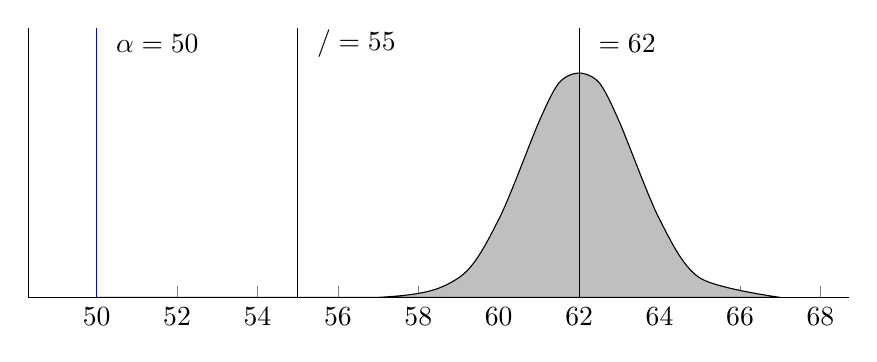
\begin{tikzpicture}
    \begin{axis}[
      axis lines*=left,
      ytick=\empty,
      height=5cm,
      width=12cm,
      enlarge y limits={value=0.2,upper},
      ]

      \draw (55, 0) -- (55, 10);
      \node at (55, 6.5) [label=right:{$\HypPopMean/ = 55$}] {};

      \draw[color=blue] (50, 0) -- (50, 10);
      \node at (50, 6.5) [label=right:{$\alpha = 50$}] {};

     \addplot[smooth, fill=lightgray, domain=40:85] 
        coordinates{
          (50, 0)
          (57, 0) (59, 0.5) (60, 2) (61, 4.5) (61.5, 5.5)
          (62, 5.75)
          (62.5, 5.5) (63, 4.5) (64, 2) (65, 0.5) (67, 0)}
        \closedcycle;

      \draw (62, 0) -- (62, 10);
      \node at (62, 6.5) [label=right:{$\populationmean = 62$}] {};

    \end{axis}
  \end{tikzpicture}
\end{center}

\noindent
If the true population mean is really centered at 62, then again, we know that any sample we could possibly take will have a mean that falls in the grey area. And since any such sample mean is greater than $\alpha$, we will conclude that such a sample mean does not provide us enough evidence to conclude that the null hypothesis should be overturned. So, we will let the null hypothesis stand.

Finally, suppose that the true population mean is far to the left of the proposed mean. For instance, suppose it is 45.

\begin{center}
  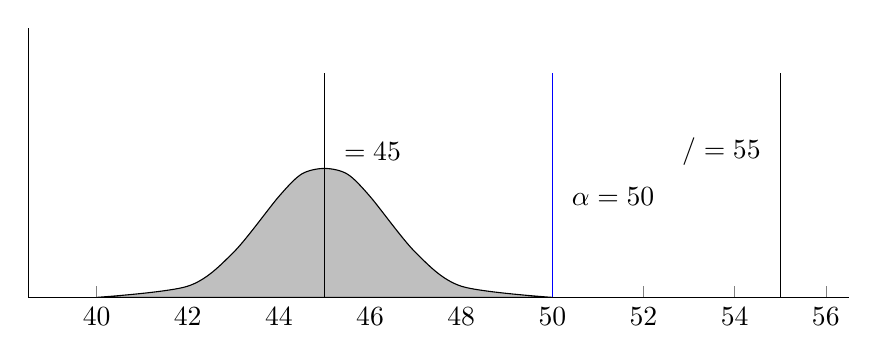
\begin{tikzpicture}
    \begin{axis}[
      axis lines*=left,
      ytick=\empty,
      height=5cm,
      width=12cm,
      enlarge y limits={value=0.2,upper},
      ]

      \draw (55, 0) -- (55, 10);
      \node at (55, 6.5) [label=left:{$\HypPopMean/ = 55$}] {};

      \draw[color=blue] (50, 0) -- (50, 10);
      \node at (50, 4.5) [label=right:{$\alpha = 50$}] {};

     \addplot[smooth, fill=lightgray, domain=40:85] 
        coordinates{
          (40, 0) (42, 0.5) (43, 2) (44, 4.5) (44.5, 5.5)
          (45, 5.75)
          (45.5, 5.5) (46, 4.5) (47, 2) (48, 0.5) (50, 0)}
        \closedcycle;

     \addplot[smooth, color=black, domain=40:85] 
        coordinates{
          (55, 0) (55, 10)}
        \closedcycle;

      \draw (45, 0) -- (45, 10);
      \node at (45, 6.5) [label=right:{$\populationmean = 45$}] {};

    \end{axis}
  \end{tikzpicture}
\end{center} 

\noindent
If the true population mean is really centered at 45, then every possible sample we could take will have a mean below $\alpha$, and so if we get any such sample, we will conclude that such a sample counts as strong enough evidence to overturn the null hypothesis.


\end{document}
